\documentclass[tikz,border=5pt]{standalone}
\usetikzlibrary{positioning}

\begin{document}
	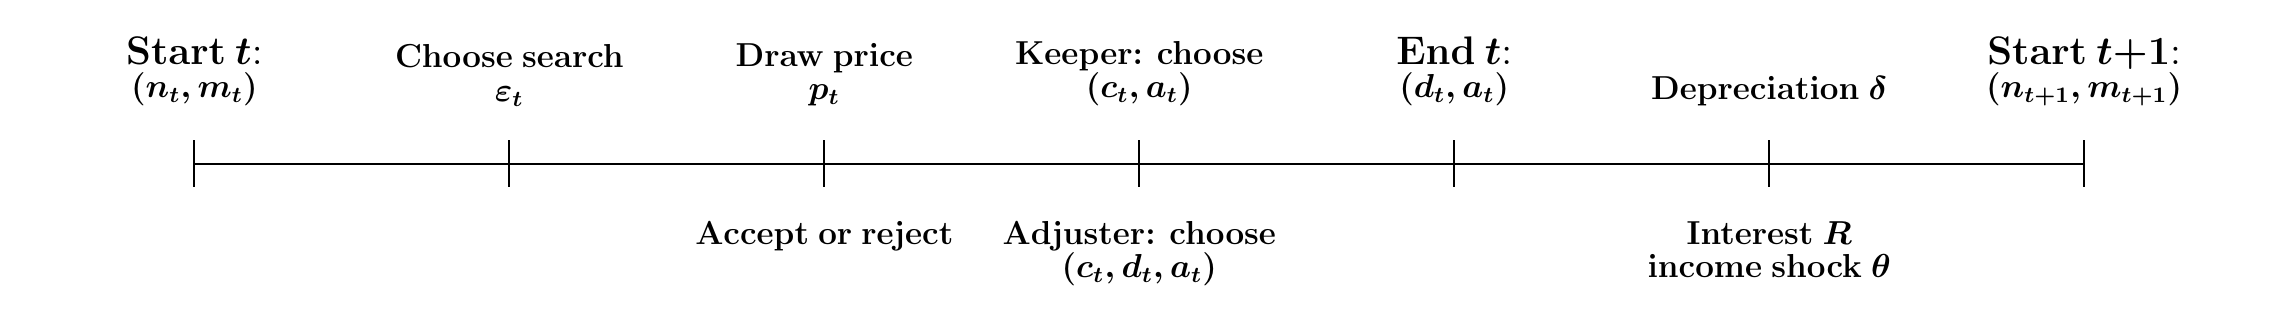
\begin{tikzpicture}[>=stealth, thick]
		
		% Timeline base
		\draw[thick] (0,0) -- (24,0);
		
		% Tick marks with alternating label placement
		\foreach \x/\pos/\label in {
			0/above/{\Large\textbf{Start \boldmath$t$}:\\ \large\textbf{\boldmath$(n_t,m_t)$}},
			4/above/{\large\textbf{Choose search} \\ \large\textbf{\boldmath$\varepsilon_t$}},
			8/above/{\large\textbf{Draw price} \\ \large\textbf{\boldmath$p_t$}},
			8/below/{\large\textbf{Accept or reject}},
			12/above/{\large\textbf{Keeper: choose} \\ \large\textbf{\boldmath$(c_t, a_t)$}},
			12/below/{\large\textbf{Adjuster: choose} \\ \large\textbf{\boldmath$(c_t, d_t, a_t)$}},
			16/above/{\Large\textbf{End \boldmath$t$}: \\ \large\textbf{\boldmath$(d_t,a_t)$}},
			20/below/{\large\textbf{Interest \boldmath$R$} \\ \large\textbf{income shock \boldmath$\theta$}},
			20/above/{\large\textbf{Depreciation \boldmath$\delta$}},
			24/above/{\Large\textbf{Start \boldmath$t{+}1$}:\\ \large\textbf{\boldmath$(n_{t+1},m_{t+1})$}}
		}{
			\draw (\x,0.3) -- (\x,-0.3); % tick
			\node[\pos=6mm, align=center, text width=4cm] at (\x,0) {\label};
		}
		
	\end{tikzpicture}
\end{document}
